
%%======%%======%0%======%%=======%%
\vspace{5mm}
\section{Problema e público alvo}
\label{sec:Publico}
%\addcontentsline{toc}{chapter}{Objetivos}

%%======%%======%0%======%%=======%%

O desenvolvimento do Site \textbf{Lab-LIFS} carrega consigo uma notável importância prática, uma vez que o grupo nunca possuiu de fato uma interface web que permitisse a integração do lab. com pessoas externas do circulo de convivência dos internos. O laboratório, atualmente, possui caráter de desenvolver pesquisas e compartilhar o uso de equipamentos presentes nas dependências do grupo. Tendo isso em vista, o aluno autor, por integrar o grupo de pesquisa, entendeu a relevância e aplicação prática de tal desenvolvimento. 

O objetivo foi portanto, criar uma interface web que permitisse de tal modo que, informações as quais antes estavam soltas, desconexas e muitas vezes difusas, agora estarão concentradas dentro de uma mesma central, de modo a facilitar bilateralmente as interações, e tornar inclusive o grupo de pesquisa mais profissional. A ideia, ao ser transmitida para o professor Dr. José R. R. Bortoleto, chefe do laboratório, foi recebida com grande alegria, entusiasmo e disposição, evidenciando que a ideia de fato sanaria um problema que é um antigo conhecido do grupo. O projeto buscou a realização das seguintes funções:
\begin{itemize}
	\item Agendamento de equipamentos e máquinas presentes no lab.;
	\item Visualização de notícias recentes e conquistas do grupo;
	\item Acesso ao acervo público de artigos, congressos, etc;
	\item Contato com alunos e professores, de modo a divulgar os trabalhos e conectar possíveis parceiros ou novos membros.
\end{itemize}


Para tal, já era entendido pelo aluno autor, que muitos usuários seriam pessoas que não são da área temática de tecnologia, mas sim na área de física ou materiais, logo, o objetivo sempre foi desenvolver uma interface responsiva, simples e prática, visto que o público alvo é outros pesquisadores da área, alunos e empresas que buscam parcerias em instituições de pesquisa tal qual a UNESP. Portanto, foi desenvolvido por meio do \textit{software} \textit{excalidraw}, um \textit{wireframe} para o projeto, de modo a melhor adequar e pegar outras referências, criando algo funcional, esteticamente agradável e moderno. A Figura \ref{fig:wireframeproject} mostra o \textit{wireframe} feito. 
\begin{figure}[H]
	\centering
	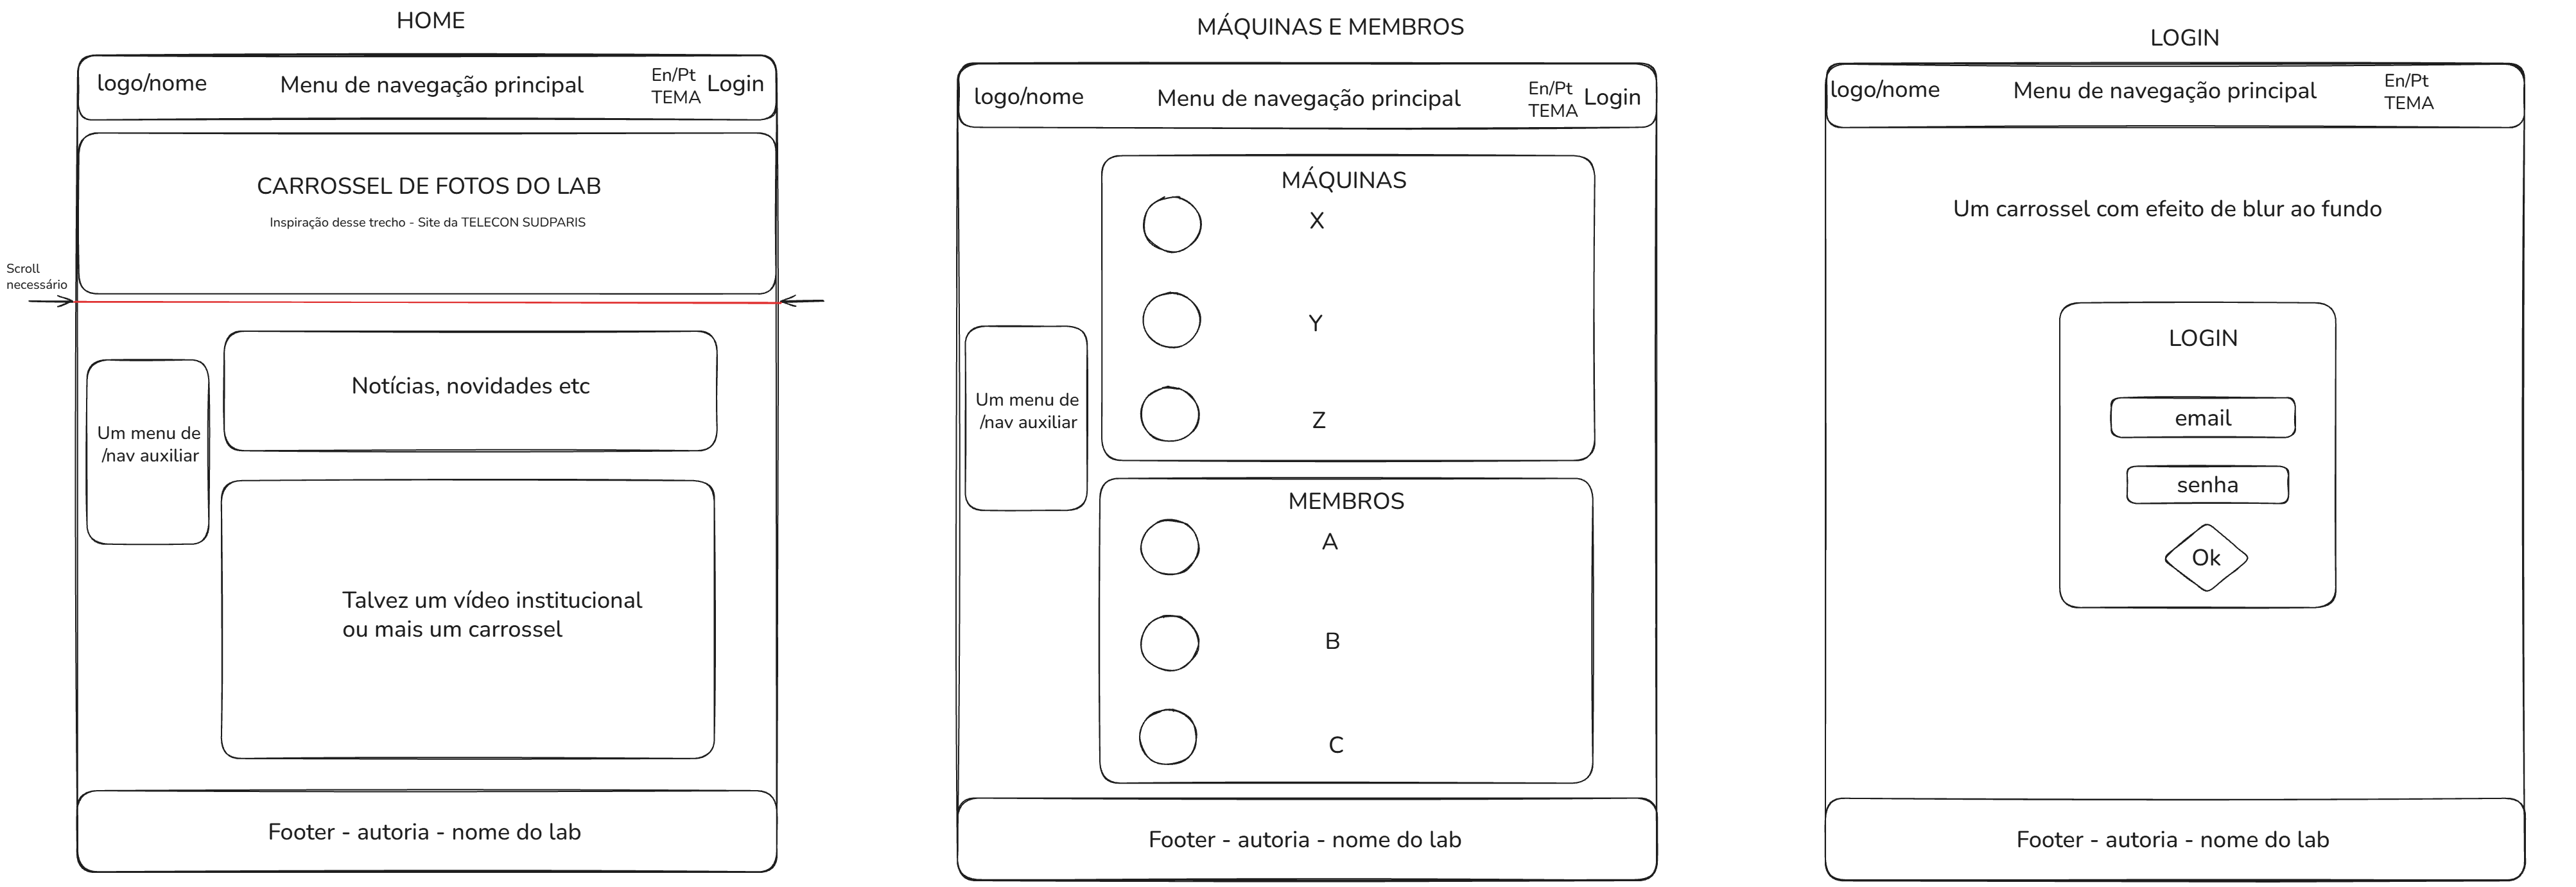
\includegraphics[width=1\linewidth]{2-imagens/wireframe_project}
	\caption{Esboço da interface idealizada para o projeto em questão.\\Fonte: O autor, 2026.}
	\label{fig:wireframeproject}
\end{figure}
